\documentclass[10pt, landscape]{article}
\usepackage[scaled=0.92]{helvet}
\usepackage{calc}
\usepackage{multicol}
\usepackage[a4paper,margin=3mm,landscape]{geometry}
\usepackage{amsmath,amsthm,amsfonts,amssymb}
\usepackage{color,graphicx,overpic}
\usepackage{hyperref}
\usepackage{newtxtext} 
\usepackage{enumitem}
\usepackage[table]{xcolor}
\usepackage{mathtools}
\setlist{nosep}
% for including images
\graphicspath{ {./images/} }

\pdfinfo{
  /Title (CS3223.pdf)
  /Creator (TeX)
  /Producer (pdfTeX 1.40.0)
  /Author (Jovyn Tan & Gavin Chiam)
  /Subject (CS3223)
/Keywords (CS3223, nus,cheatsheet,pdf)}

% Turn off header and footer
\pagestyle{empty}

% redefine section commands to use less space
\makeatletter
\renewcommand{\section}{\@startsection{section}{1}{0mm}%
  {-1ex plus -.5ex minus -.2ex}%
  {0.5ex plus .2ex}%x
{\normalfont\large\bfseries}}
\renewcommand{\subsection}{\@startsection{subsection}{2}{0mm}%
  {-1explus -.5ex minus -.2ex}%
  {0.5ex plus .2ex}%
{\normalfont\normalsize\bfseries}}
\renewcommand{\subsubsection}{\@startsection{subsubsection}{3}{0mm}%
  {-1ex plus -.5ex minus -.2ex}%
  {1ex plus .2ex}%
{\normalfont\small\bfseries}}%
\makeatother

\renewcommand{\familydefault}{\sfdefault}
\renewcommand\rmdefault{\sfdefault}
%  makes nested numbering (e.g. 1.1.1, 1.1.2, etc)
\renewcommand{\labelenumii}{\theenumii}
\renewcommand{\theenumii}{\theenumi.\arabic{enumii}.}
\renewcommand\labelitemii{•}
\renewcommand\labelitemiii{•}

\definecolor{mathblue}{cmyk}{1,.72,0,.38}
\everymath\expandafter{\the\everymath \color{mathblue}}

% Don't print section numbers
\setcounter{secnumdepth}{0}

\setlength{\parindent}{0pt}
\setlength{\parskip}{0pt plus 0.5ex}
%% adjust spacing for all itemize/enumerate
\setlength{\leftmargini}{0.5cm}
\setlength{\leftmarginii}{0.5cm}
\setlist[itemize,1]{leftmargin=2mm,labelindent=1mm,labelsep=1mm}
\setlist[itemize,2]{leftmargin=4mm,labelindent=1mm,labelsep=1mm}
\setlist[itemize,3]{leftmargin=4mm,labelindent=1mm,labelsep=1mm}

% adding my commands
% tightcenter
\newenvironment{tightcenter}{%
  \setlength\topsep{0pt}
  \setlength\parskip{0pt}
  \begin{center}
    }{%
  \end{center}
}

% boxed
\newenvironment{tightbox}{%
  \setlength\topsep{0pt}
  \setlength\parskip{0pt}
  \begin{center}
    \begin{tabular}{|@{\hspace{\dimexpr\fboxsep+0.5\arrayrulewidth}}c@{\hspace{\dimexpr\fboxsep+0.5\arrayrulewidth}}|}
      \hline
    }
    {%
    \\ \hline
    \end{tabular}
  \end{center}
}

% fixed width box
\newenvironment{fixedbox}[1][0.7]{
  \setlength\topsep{0pt}
  \setlength\parskip{0pt}
  \begin{center}
    \begin{tabular}{|>{\centering\arraybackslash}m{#1\linewidth}|}
    \hline
  }{
  \\ \hline
  \end{tabular}
  \end{center}
}

% definition of a new term
\usepackage{soul}
\definecolor{paleyellow}{RGB}{251,243,218}
\newcommand{\definition}[2][]{\sethlcolor{paleyellow}\hl{\textbf{#2}} #1  $\rightarrow$}

% important note (attention)
\newcommand{\attention}{{\color{red}\textbf{! }}}



% -----------------------------------------------------------------------

\begin{document}
\raggedright
\footnotesize
\begin{multicols*}{4}
  % multicol parameters
  \setlength{\columnseprule}{0.25pt}

  \begin{center}
    \fbox{%
      \parbox{0.8\linewidth}{\centering \textcolor{black}{
          {\Large\textbf{CS3223}}
        \\ \normalsize{AY23/24 SEM 2}}
      }%
    }
  \end{center}

  \section{01. DBMS STORAGE}

  \begin{itemize}
    \item store data on non-volatile disk
    \item process data in main memory (RAM) (\textit{volatile storage})
  \end{itemize}  

  \subsection{Magnetic HDD}

  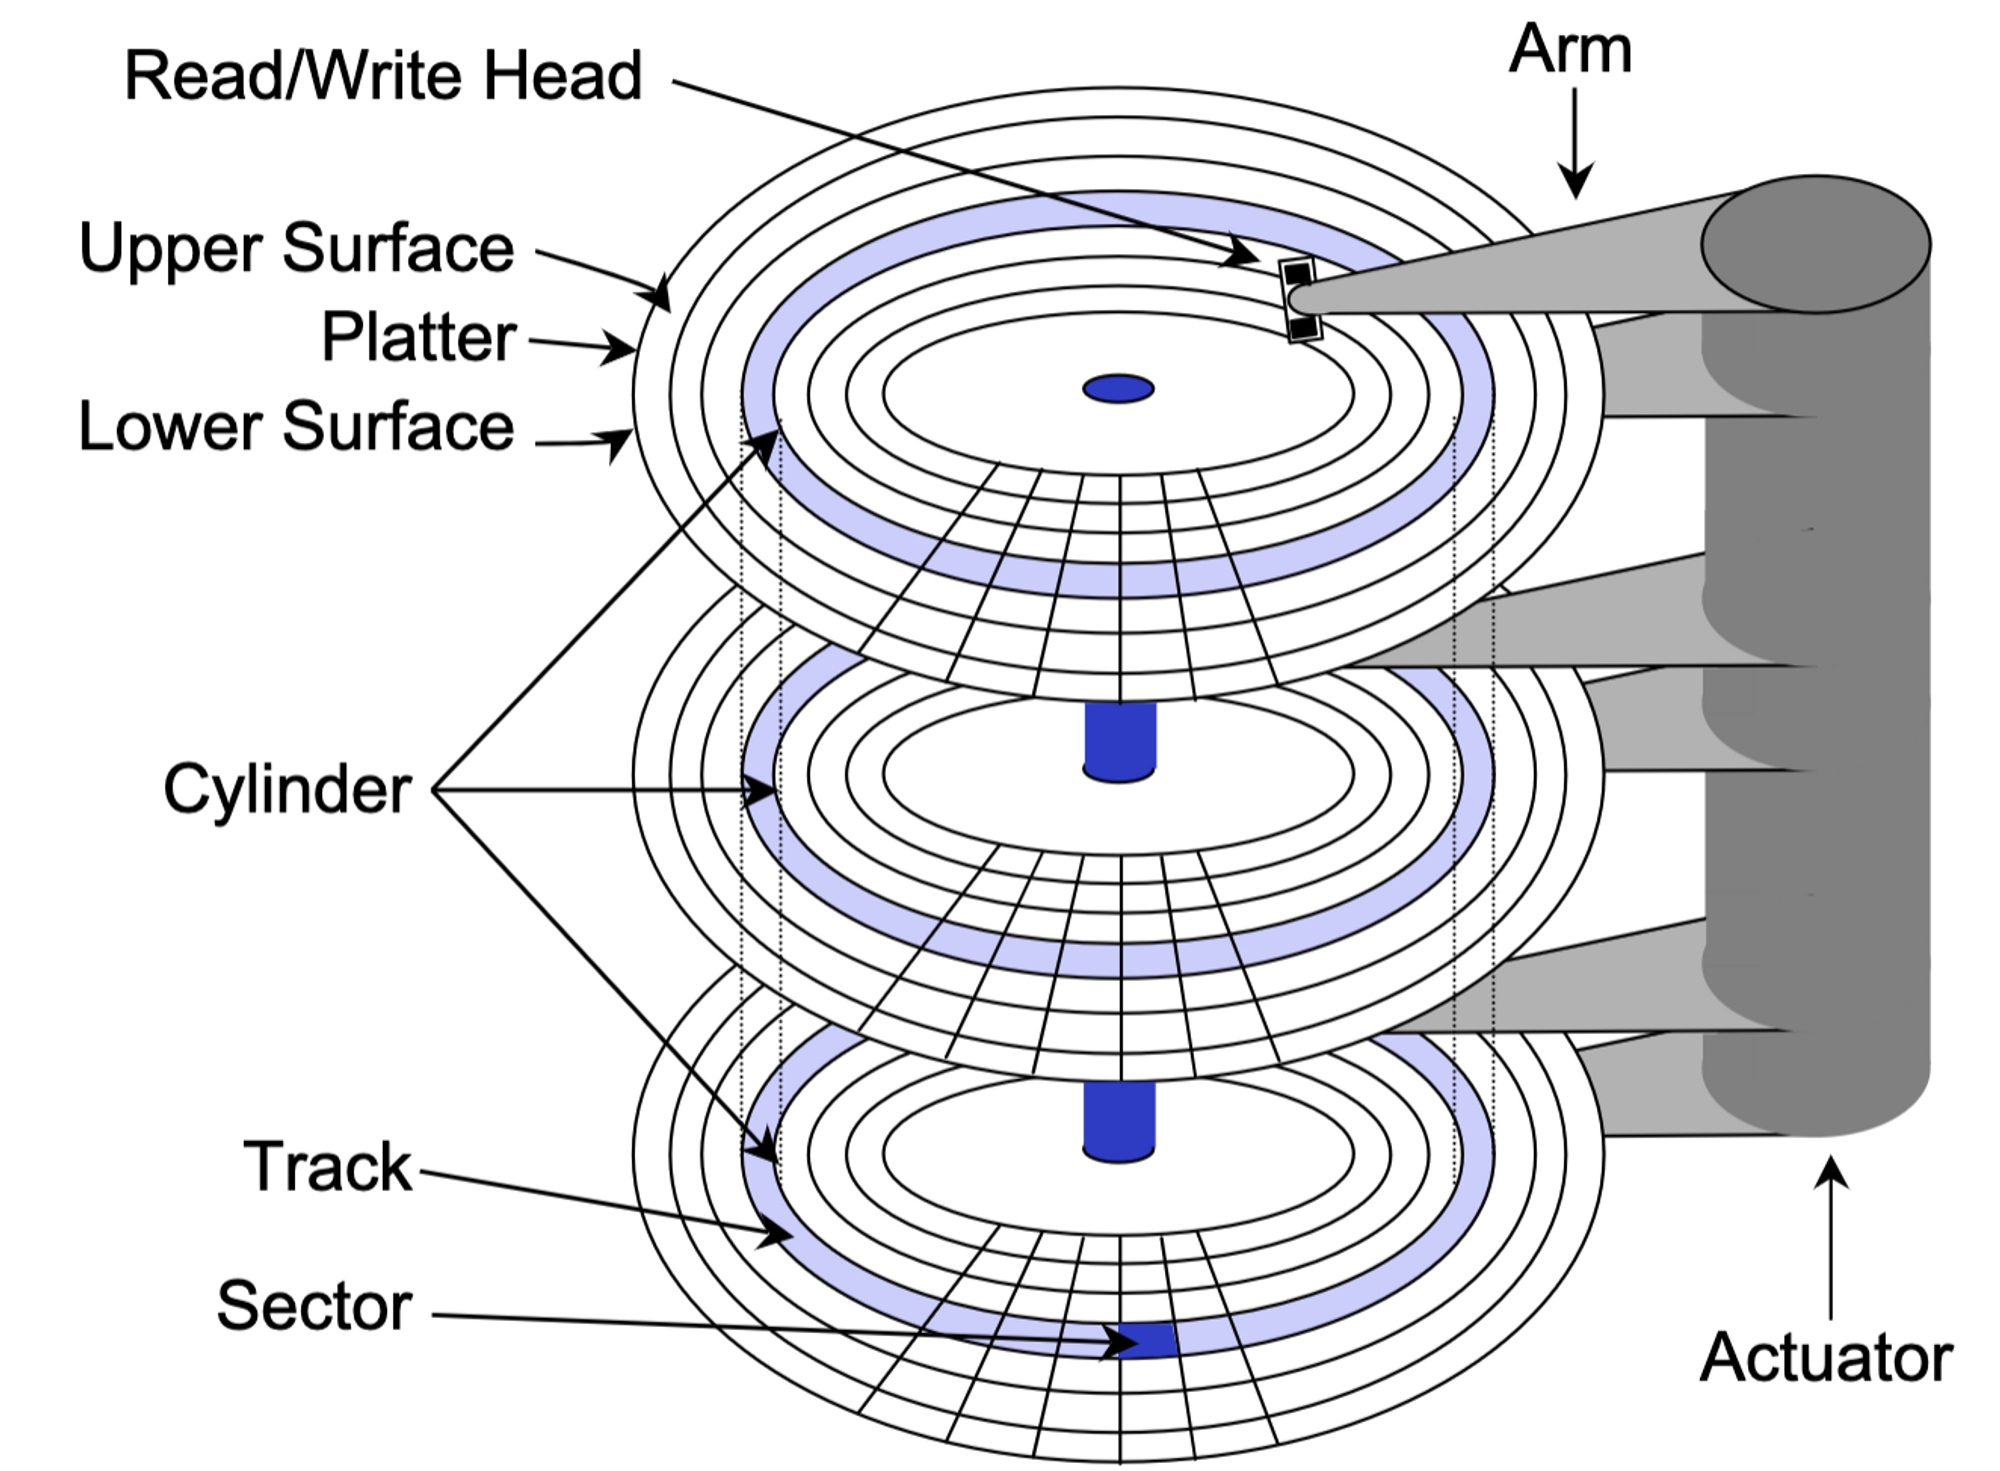
\includegraphics[width=0.9\linewidth]{cs3223-magnetic-hdd.png} 

  \begin{itemize}
    \item \textbf{disk access time} =
      \begin{itemize}
        \item \definition{seek time} move arms to position disk head on track.
          \\$\text{Total(sequential)} = \text{num of cylinders} \times \text{seek time}$
        \item \definition{rotational delay} wait for block to rotate under head
          \begin{itemize}
            \item average rotational delay = time for $\frac{1}{2}$ revolutions
            \item $ = 0.5 \times \frac{60}{\text{rotational speed (RPM)}}$
          \end{itemize}
        \item \definition{transfer time} move data to/from disk surface
          \\* $= \text{time for 1 revolution} \times \frac{ \text{\# of requested sectors on the same track} }{ \text{\# of sectors in track} } $
      \end{itemize}
    \item \textbf{response time} for disk access = queuing delay+access time
  \end{itemize}

  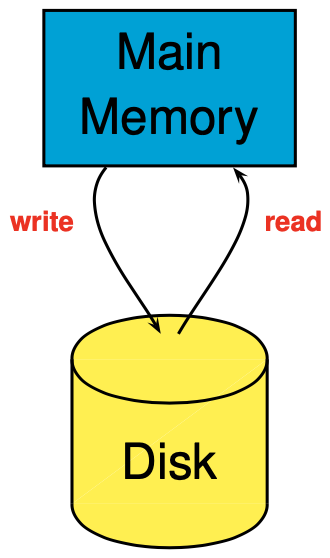
\includegraphics[width=0.15\linewidth]{cs3223-dbms-storage.png} 
  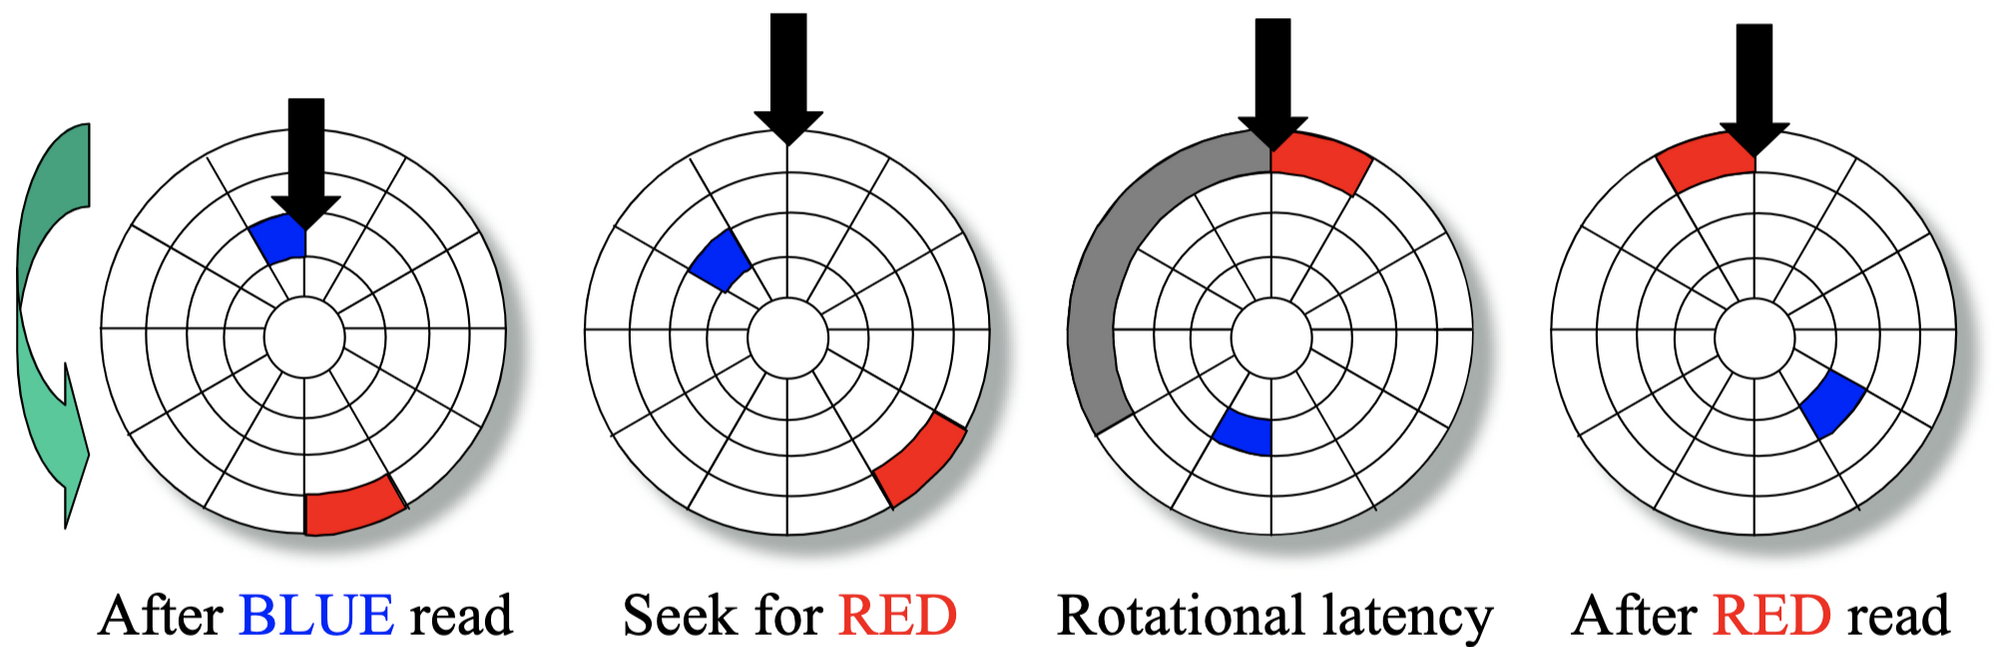
\includegraphics[width=0.8\linewidth]{cs3223-access-time-example.png} 

  \begin{itemize}
    \item command processing time: interpreting access command by disk controller (part of access time, considered negligible)
    \item small requests are dominated by seek time; large requests dominated by transfer time
    \item \textbf{access order}:
      \begin{enumerate}
        \item contiguous blocks within the same track (same surface)
        \item cylinder tracks within the same cylinder
        \item next cylinder
      \end{enumerate}
  \end{itemize}

  \subsection{SSD (Solid-State Drive)}

  \begin{itemize}
    \item no mechanical moving parts
    \item advantages: $\checkmark$ significantly faster than HDD \\* $\checkmark$ higher data transfer rate $\checkmark$ lower power consumption
    \item disadvantages: $\times$ update to a page requires erasure of multiple pages before overwriting page \\*
      $\times$ limited number of times a page can be erased
  \end{itemize} 

  \subsection{Buffer Manager}

  \begin{itemize}
    \item data is stored \& retrieved in \textbf{disk blocks} (pages)
      \begin{itemize}
        \item each block = sequence of $\geq 1$ contiguous sectors
      \end{itemize}
    \item \textbf{buffer pool}: main memory allocated for DBMS
      \begin{itemize}
        \item partitioned into \ildefinition{frames} (block-sized pages)
      \end{itemize}
    \item \textbf{\texttt{pin count}}: number of clients using page (initialised 0)
      \begin{itemize}
        \item $> 0 \Rightarrow$ page is utilised by some transaction; don't replace
      \end{itemize}
    \item \textbf{\texttt{dirty} flag}: initialised false
      \begin{itemize}
        \item \definition{dirty} page is modified \& not updated on the disk
        \item dirty page must be written back to the disk if the transaction has committed
      \end{itemize}
  \end{itemize}

  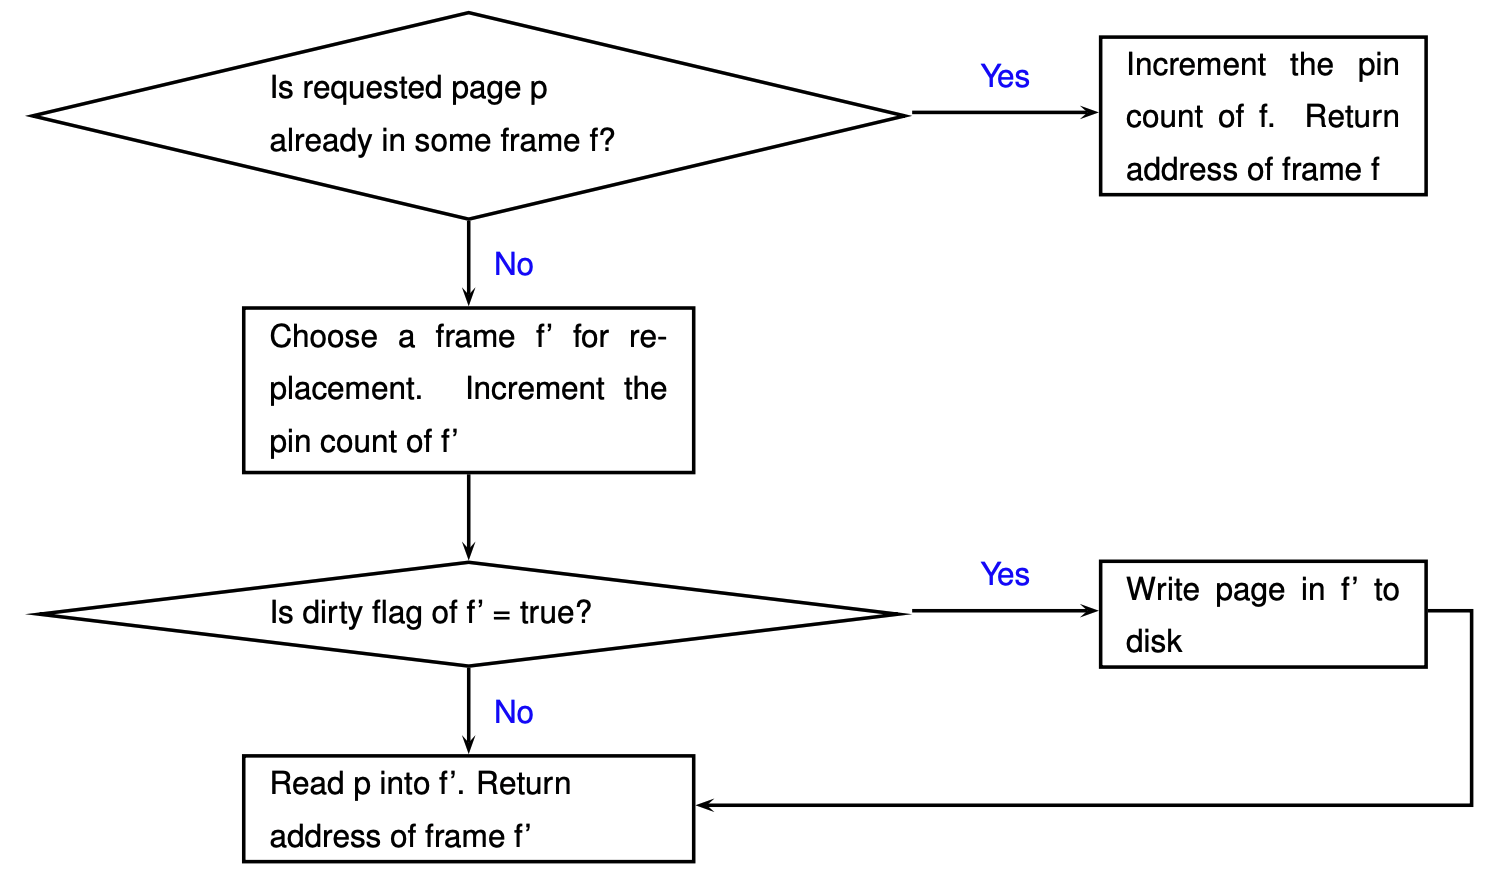
\includegraphics[width=0.95\linewidth]{cs3223-buffer-manager-request-handling.png} 

  \attention unpinning: update dirty flag to true if page is dirty

  \subsubsection{replacement policies}

  \begin{itemize}
    \item decide which unpinned (\texttt{pinCount==0}) page to replace
    \item \textbf{LRU} uses a queue of pointers to frames with \texttt{pinCount==0}
    \item \textbf{clock}: cheaper than LRU, used in postgres
      \begin{itemize}
        \item \texttt{referenced bit} - turns on when \texttt{pinCount==0}
        \item replace page with referenced bit off \texttt{\&\& pinCount==0}
      \end{itemize}
      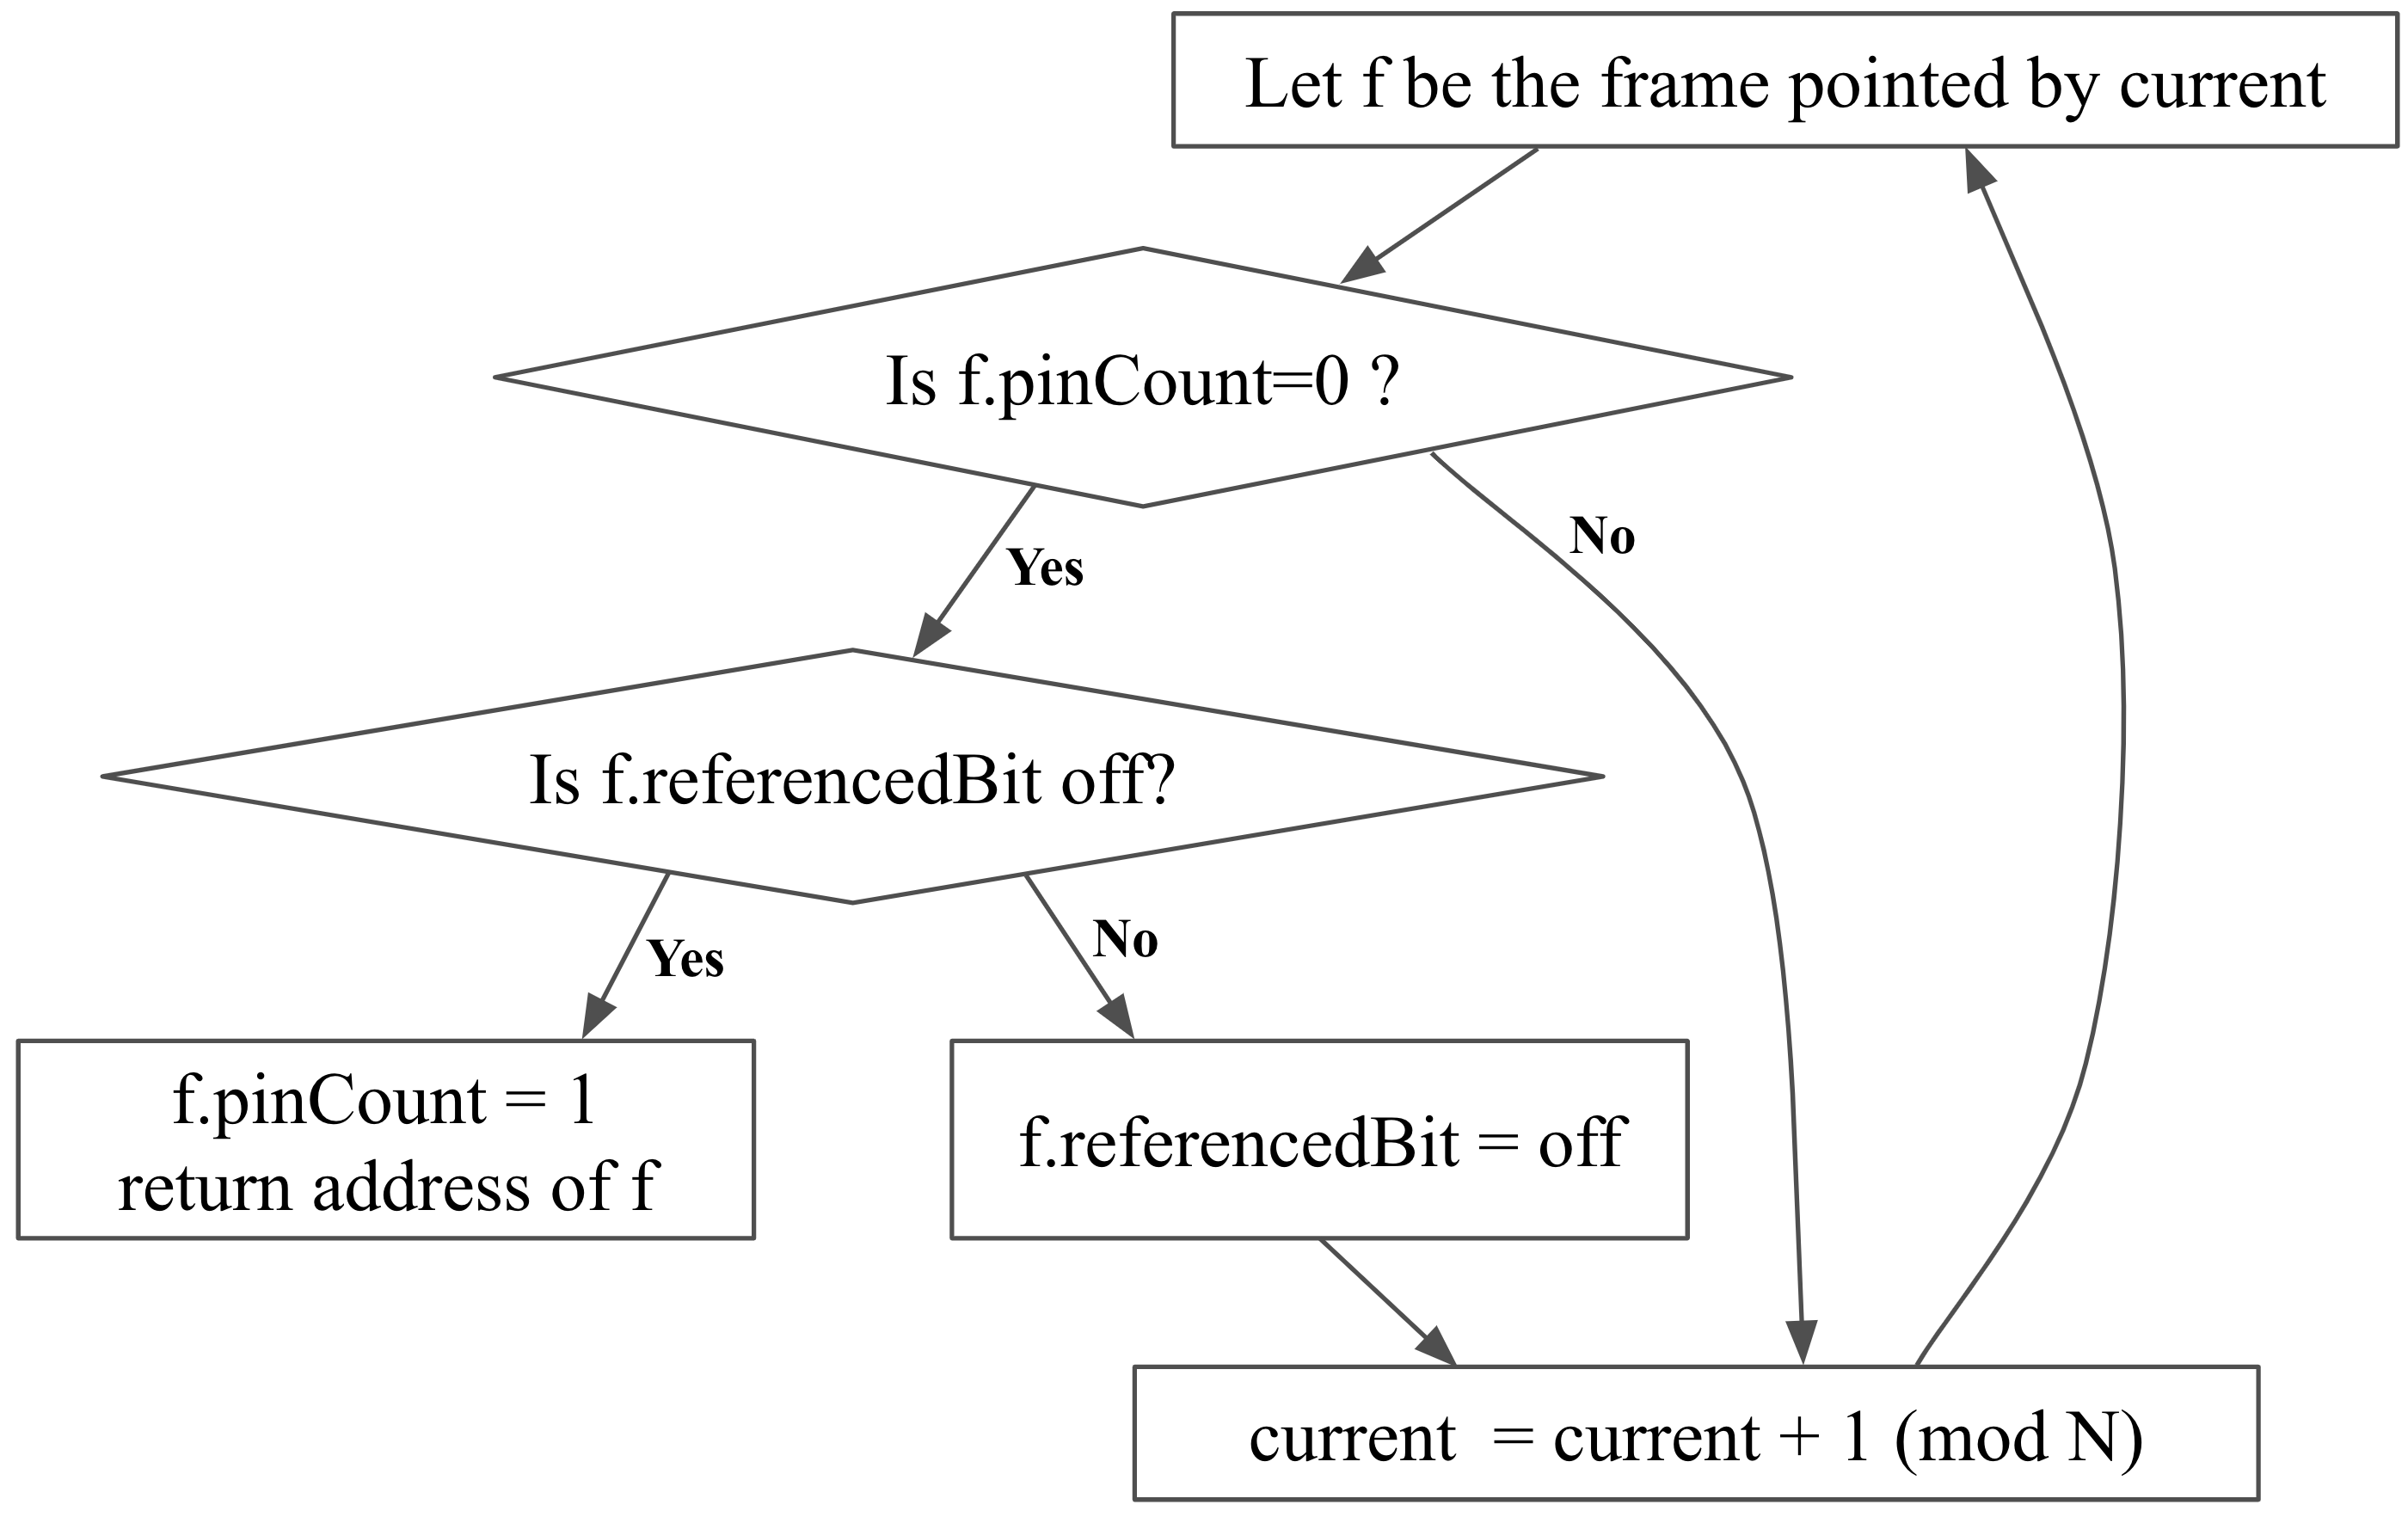
\includegraphics[width=0.85\linewidth]{cs3223-clock-replacement-policy.png} 
  \end{itemize}

  \subsection{File abstraction}

  \begin{itemize}
    \item each relation is a file of records
    \item each record has a unique record identifier, \ildefinition{RID}
    \item \definition{heap file} unordered file
      \begin{itemize}
        \item vs sorted/hashed file: records are ordered/hashed
      \end{itemize}
  \end{itemize}

  \subsubsection{heap file implementations}

  \begin{itemize}
    \item \textbf{linked list} implementation
      \begin{itemize}
        \item header page: metadata about the file
          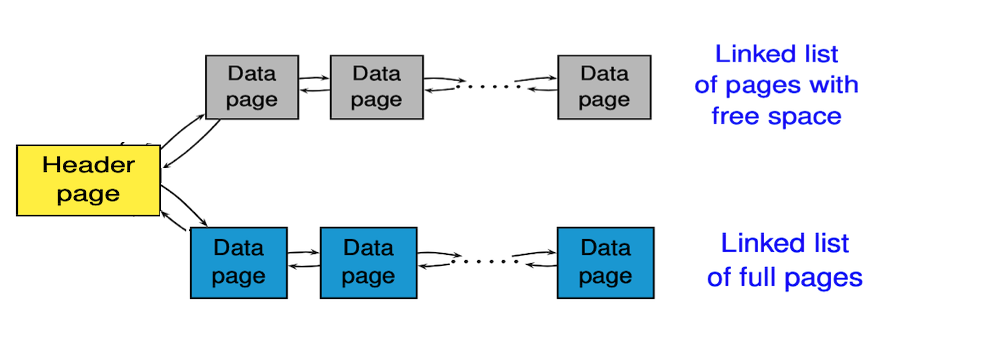
\includegraphics[width=0.75\linewidth]{cs3223-file-linked-list.png} 
      \end{itemize}
    \item \textbf{page directory} implementation: more efficient
      \begin{itemize}
        \item maintain directory structure with one entry per page 
          \begin{itemize}
            \item stores address of and amount of free space on page
          \end{itemize}
        \item insertion: scan directory to find page with enough space to store the new record
        \item insertion worst case: scan number of pages + data page itself (vs LL worst case: entire list)
          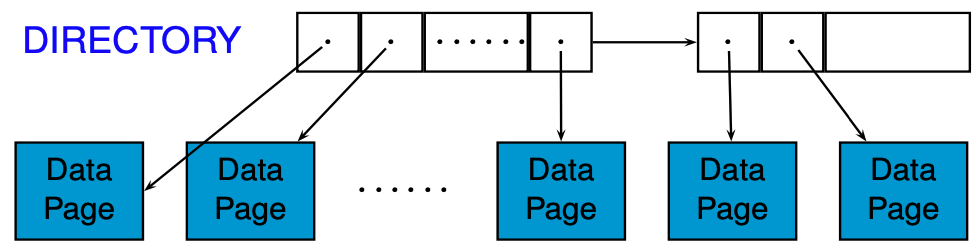
\includegraphics[width=0.6\linewidth]{cs3223-file-page-directory.png} 
      \end{itemize}
  \end{itemize}

  \subsection{Page Formats}

  \begin{itemize}
    \item \texttt{RID} = (page ID, slot number)
    \item \textbf{fixed-length} records
      \begin{itemize}
        \item packed organisation: inefficient deletion (transferring last record to deleted record changes RID of record)
      \end{itemize}
    \item \textbf{variable-length} records: \textbf{slotted page organisation}
  \end{itemize}

  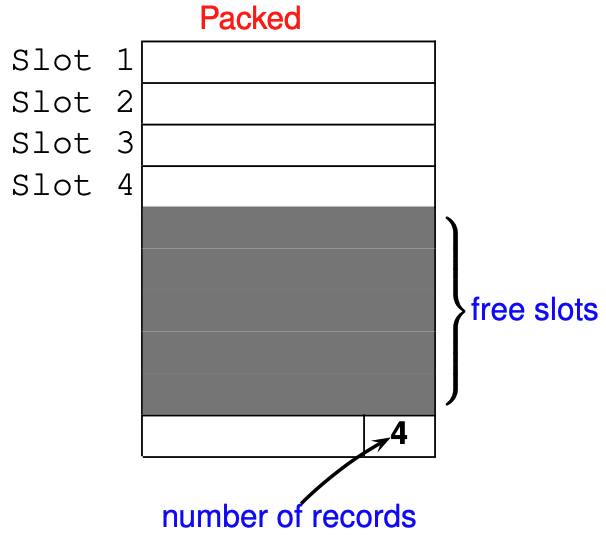
\includegraphics[width=0.3\linewidth]{cs3223-packed-organisation.png} 
  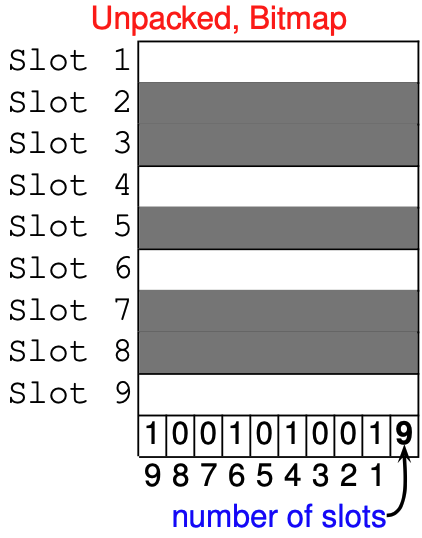
\includegraphics[width=0.2\linewidth]{cs3223-unpacked-organisation.png} 
  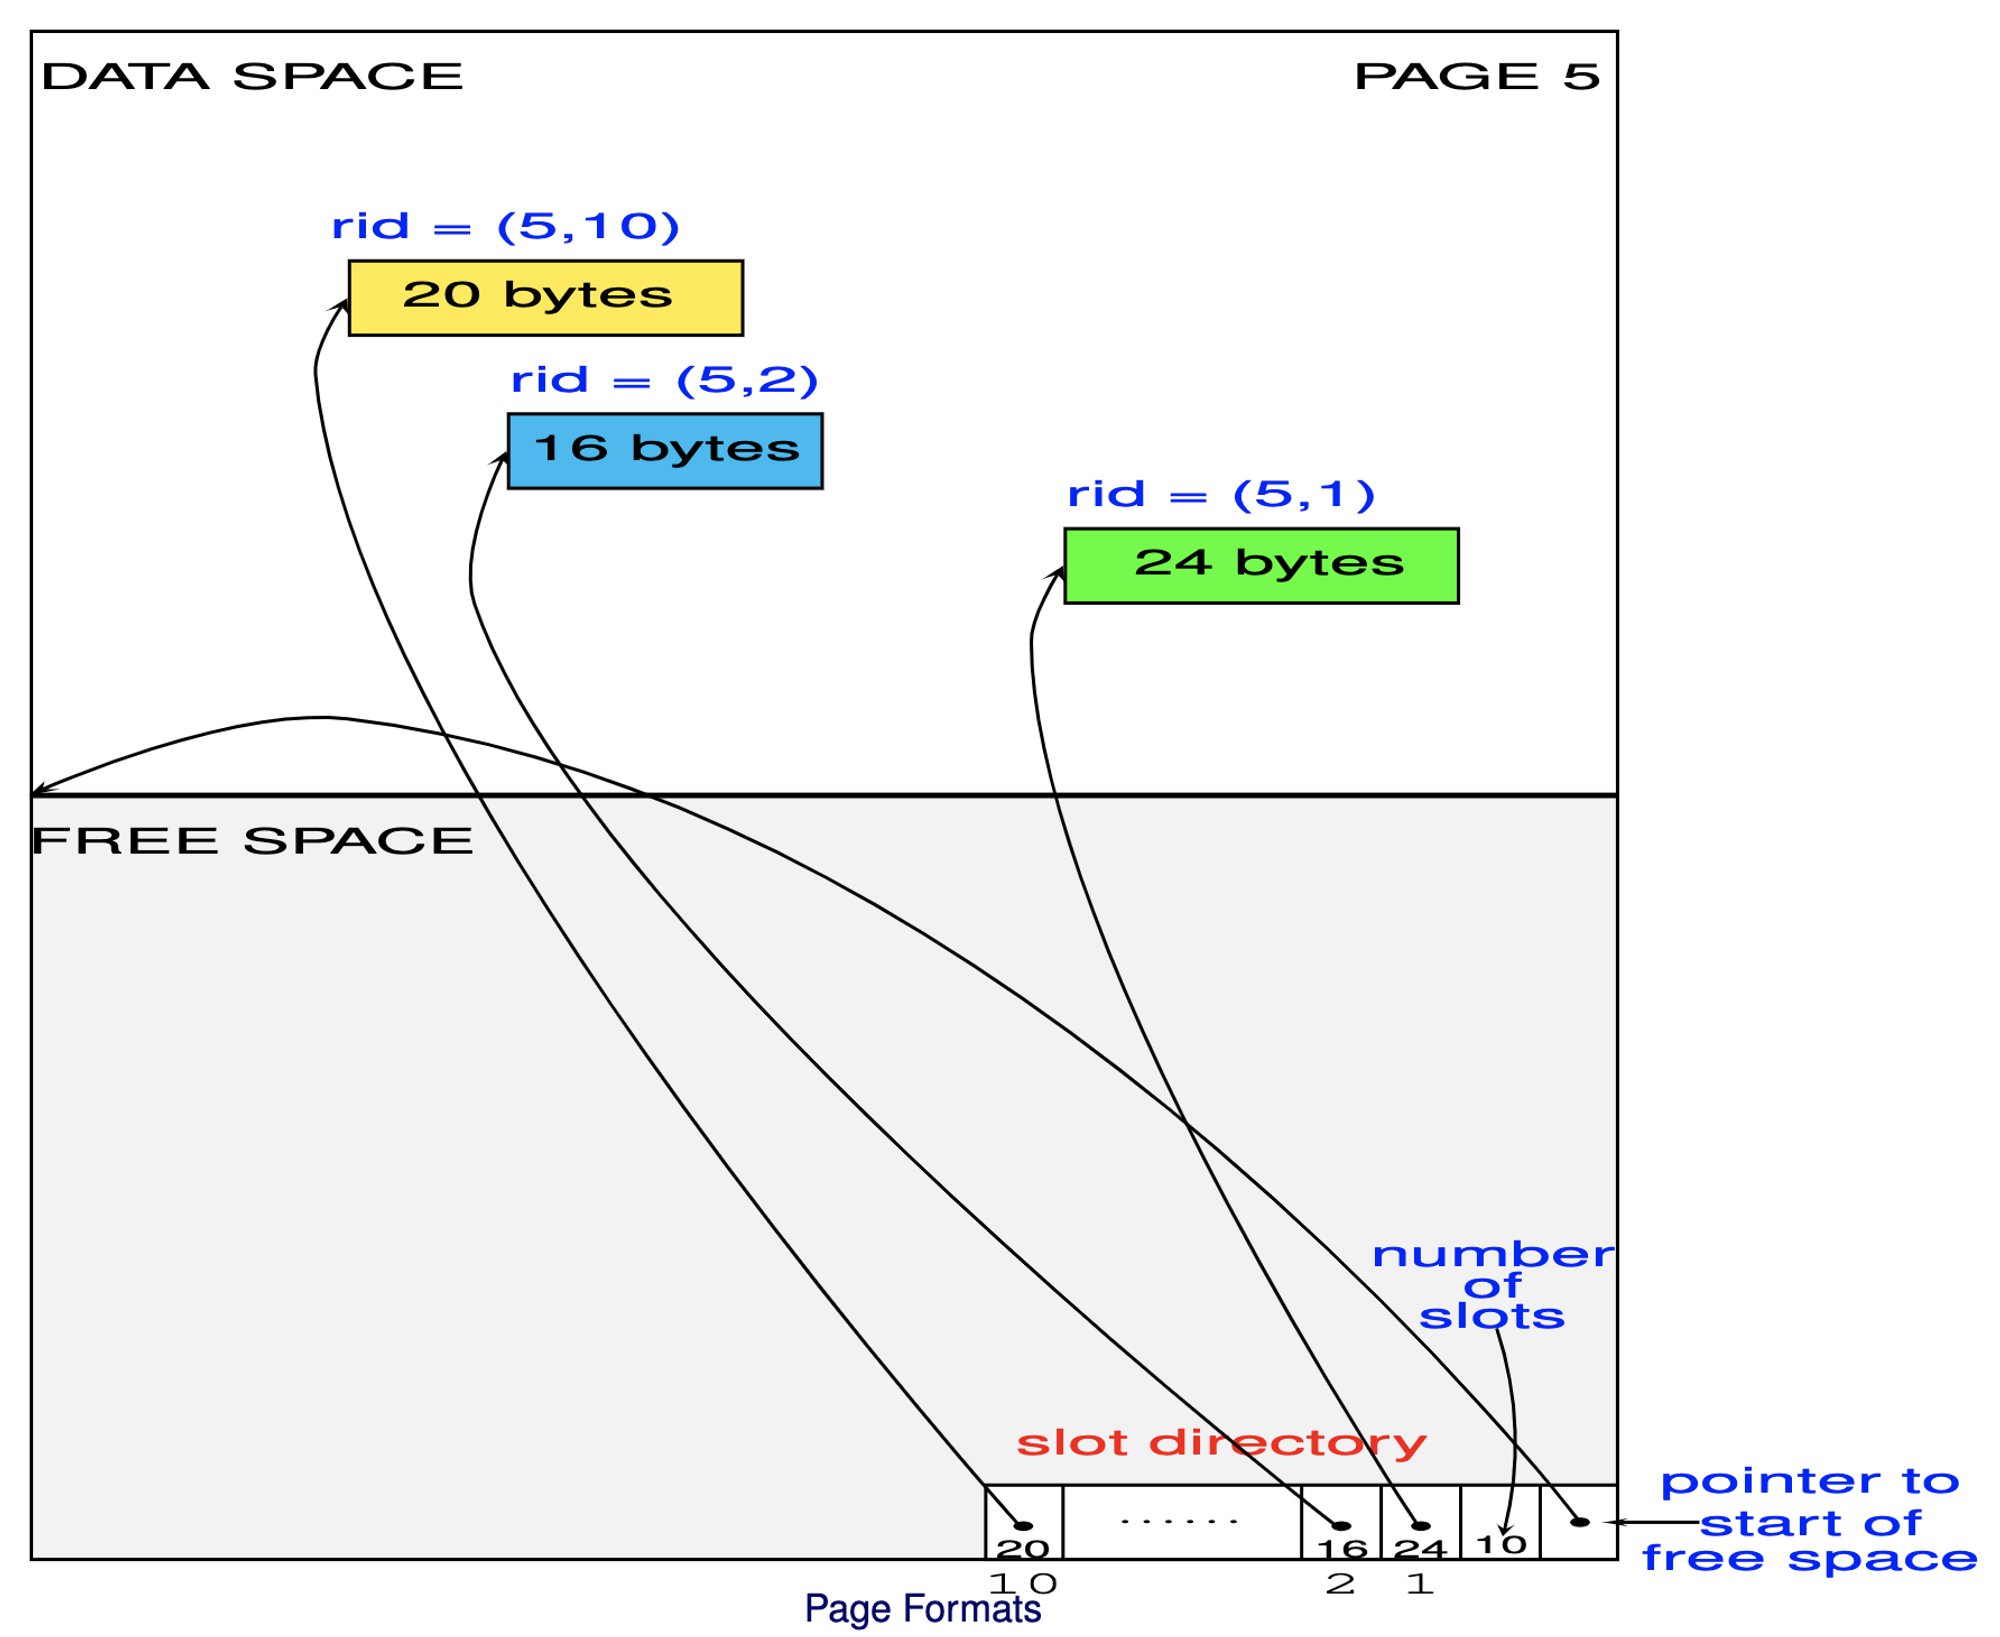
\includegraphics[width=0.46\linewidth]{cs3223-slotted-page-organisation.png} 

  \subsubsection{Record formats}

  \begin{itemize}
    \item \textbf{fixed-length} records: store consecutively
    \item \textbf{variable-length} records:
      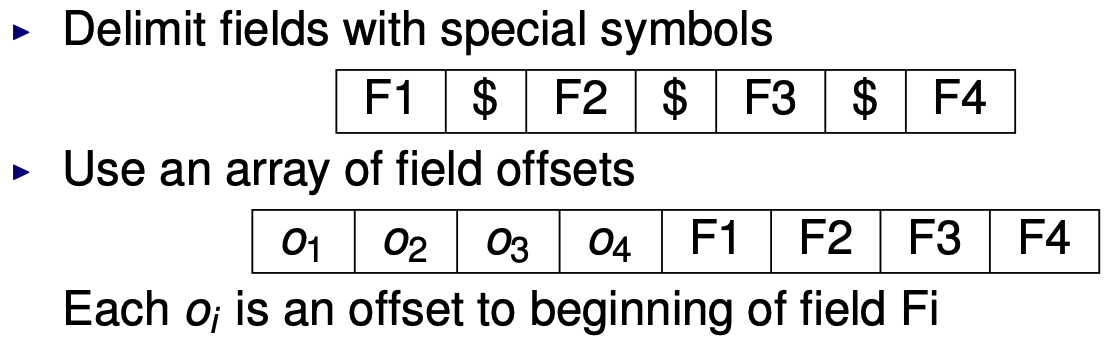
\includegraphics[width=0.7\linewidth]{cs3223-variable-length-records.png}
  \end{itemize}

  \subsubsection{Data entry formats}

  \begin{enumerate}
    \item k* is an actual \textbf{data record} (with search key $k$) 
    \item k* is of the form \textbf{(k, RID)} - fixed length \texttt{(k, \textbf{$\bullet$})}
    \item k* is of the form \textbf{(k, RID-list)} - e.g. (k, \{RID11, RID12\})
  \end{enumerate}

  \section{02. TREE-BASED INDEXING}

  \begin{itemize}
    \item \definition{search key} sequence of $k$ data attributes, $k \geq 1$ 
      \begin{itemize}
        \item \definition{composite search key} if $k > 1$
      \end{itemize}
    \item \definition{unique index} search key is a candidate key
    \item \definition{clustered index} order of data entries $\approx$ order of records
      \begin{itemize}
        \item \textbf{Format-1} is \textit{always clustered}
        \item \textit{at most one} clustered index for each relation
      \end{itemize}
    \item \definition{dense index} there is an index record for every search key value in the data. \textit{unclustered index} must be dense
  \end{itemize}


  \subsection{B$^+$-tree Index}

  \begin{itemize}
    \item leaf nodes: sorted data entries ($k^*$ is of form \texttt{(k, RID)})
    \item internal nodes: stores index entries $(p_0, k_1, p_1, \dots, p_n)$ for $k_1 < k_2 \dots <k_n$ where $p_i$ is the page disk address
      \begin{itemize}
        \item each $(k_i, p_i)$ is an \textbf{index entry}
        \item for $k*$ in index subtree $T_i$ rooted at $p_i$, $k \in [k_i, k_{i+1}]$
      \end{itemize}
    \item \ildefinition{order} of index tree, $d \in \mathbb{Z}^+$
      \begin{enumerate}
        \item each non-root node contains $m$ entries, $m \in [d, 2d]$
        \item root node contains $[1, 2d]$ entries
      \end{enumerate}
    \item \textbf{equality search}: at each internal node $N$, find the largest $k_i$ s.t. $k \geq k_i$. search subtree at $p_i$ if $k_i$ exists, else $p_0$ 
    \item \textbf{range search}: find first matching record; traverse doubly LL
      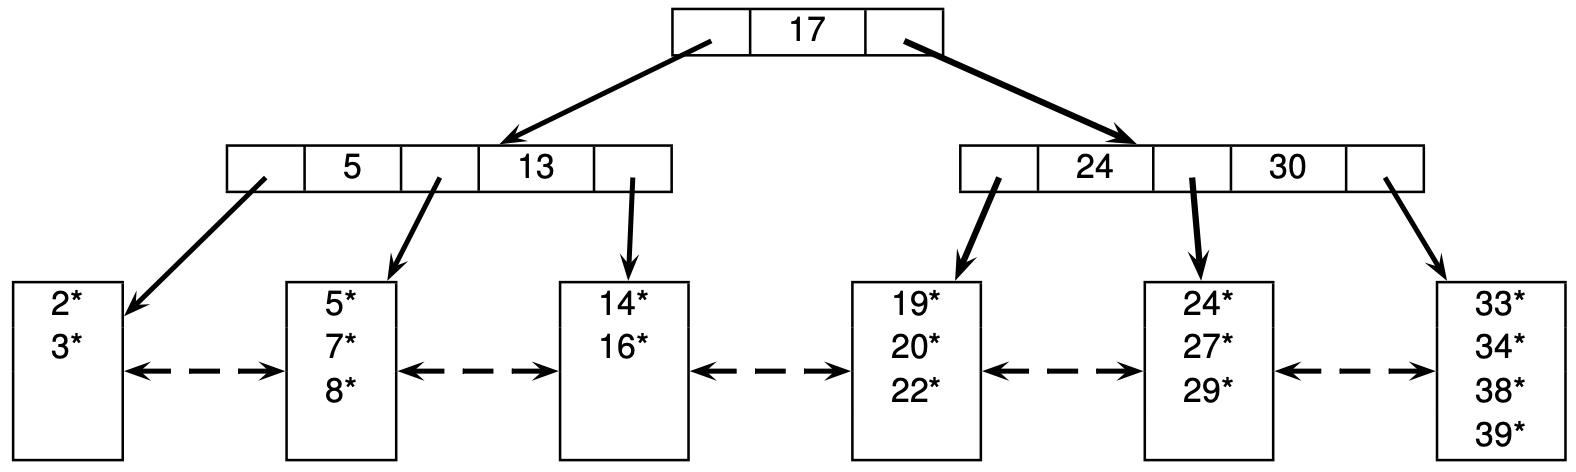
\includegraphics[width=0.9\linewidth]{cs3223-b-tree.png} 
  \end{itemize}

  \textbf{insertion: splitting}
  \begin{itemize}
    \item splitting leaf node: distribute $d+1$ entries to a new leaf node
    \item if parent overflows: push the middle (d+1) key up to parent
    \item root node overflows: create new root (parent of current root)
  \end{itemize}

  \textbf{insertion: redistribution} (of \textit{leaf nodes only})
  \begin{itemize}
    \item try right sibling first, then left sibling, else use splitting
    \item \definition{sibling} two nodes at the \textit{same level} \& \textit{same parent node}
  \end{itemize}

  \textbf{deletion: redistribution} - try right sibling, then left, else merge

  \textbf{deletion: merging} (siblings have $d$ entries) - try right first 
  \begin{itemize}
    \item if leaf underflows: delete parent key, combine with sibling
    \item if internal node underflows: pull down its index entry in parent, combine with sibling, push a key back up
      \begin{itemize}
        \item becomes the new root if parent is root \& becomes empty
      \end{itemize}
  \end{itemize}

  \textbf{finding order of $B^+$ tree with page byte size} \\$\geq 2d(\text{key byte size}) + (2d+1)(\text{disk page addr byte size})$

  \textbf{min number of nodes at level i} \\$= 2 \times (d+1)^{i-1} \text{ for } i \geq 1$

  \textbf{max number of nodes at level i} \\$= (2d+1)^i$

  \subsection{Bulk Loading a B$^+$-tree}

  \begin{enumerate}
    \item sort data entries by search key and store sequentially
    \item construct leaf pages with $2d$ entries
    \item construct internal pages by attempting to insert leaf pages into rightmost parent page
  \end{enumerate}

  \section{03. HASH-BASED INDEXING}

  \subsection{Static Hashing}

  \begin{itemize}
    \item hash record to $B_i \in B_0, \dots, B_{N-1}$ with $i = h(k)mod\, N$
    \item when full, reconstruct hash table with more buckets
  \end{itemize}
  \begin{minipage}[c]{0.55\linewidth}
    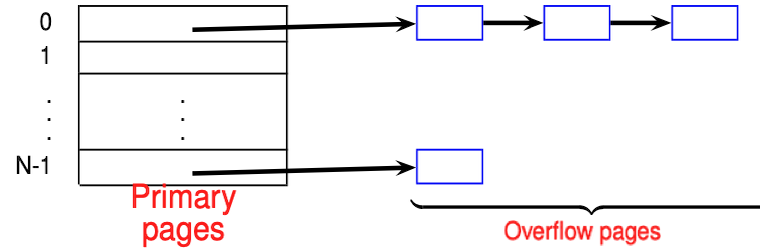
\includegraphics[width=0.95\linewidth]{cs3223-hash-bucket-pages.png} 
  \end{minipage}
  \begin{minipage}[c]{0.42\linewidth}
    each bucket:
    \begin{itemize}
      \item 1 primary data page
      \item $\geq 0$ overflow data pages
    \end{itemize}
  \end{minipage}

  \subsection{Linear Hashing (Dynamic)}

  \begin{itemize}
    \item grows \textbf{linearly}: split when some \textbf{bucket overflows}
    \item how to split bucket $B_i$ : 
      \begin{enumerate}
        \item add a new bucket $B_j = B_{i+N_i}$ (\textit{split image} of $B_i$)
        \item redistribute entries in $B_i$ between $B_i$ and $B_j$
        \item \texttt{next++}; if next==$N_{level}$: \texttt{level++; next=0}
      \end{enumerate}
    \item file size at the beginning of round $i$, $N_i = 2^iN_0$
    \item at round $i$, hash $x$ = $B_x$ has been split ? $h_i(k)$ : $h_{i+1}(k)$
    \item $N_0=2^m; N^i=2^{m+i};$
    \item Look at $m+i+1$ bits if bucket has been split, $m+i$ bits only otherwise
  \end{itemize}
  \begin{minipage}[c]{0.6\linewidth}{\textcolor{black}{
        \begin{itemize}
          \item \textbf{performance}: 1 disk I/O \\* (no overflow pages)
            \begin{itemize}
              \item avg 1.2 I/Os (uniform distribn), worst case linear I/O cost
            \end{itemize}
          \item removing last bucket (\textbf{deletion}): 
            \begin{itemize}
              \item if next $>$ 0: \texttt{next-{}-;}
              \item else: \texttt{next=}(prev level last bucket); \texttt{level-{}-;}
            \end{itemize}
        \end{itemize}
    }}
  \end{minipage}
  \begin{minipage}[c]{0.37\linewidth}
    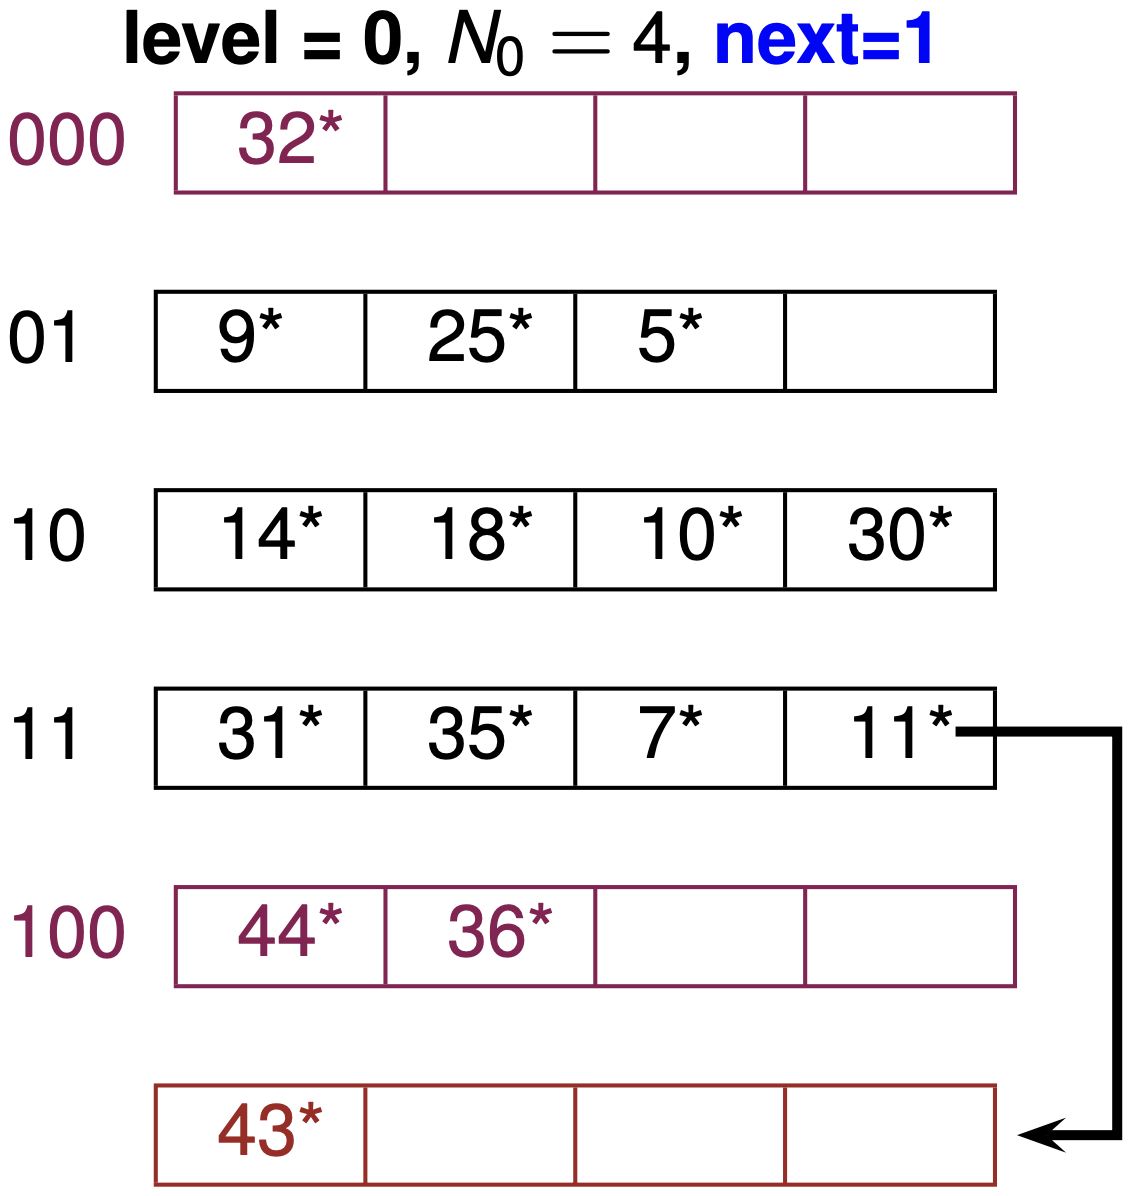
\includegraphics[width=0.95\linewidth]{cs3223-linear-hashing.png} 
  \end{minipage}

  \subsection{Extendible Hashing (Dynamic)}

  \begin{itemize}
    \item add a new bucket whenever existing bucket overflows 
      \begin{itemize}
        \item no overflow pages unless \# collisions $>$ page capacity 
      \end{itemize}
    \item directory of pointers to buckets - $2^d$ entries ($b_db_{d-1}\dots b_1$)
      \begin{itemize}
        \item $d=$ \ildefinition{global depth} of hashed file
      \end{itemize}
    \item \ildefinition{corresponding} directory entries differ only in the $d^{th}$ bit
    \item entries in a bucket of \ildefinition{local depth} $\ell \in [0,d]$: same last $\ell$ bits
      \begin{itemize}
        \item a split bucket \& its image have the \textit{same local depth}
      \end{itemize}
    \item number of directory entries pointing to a bucket = $2^{d-\ell}$
    \item Look at last $\ell$ bits when adjusting pointers
      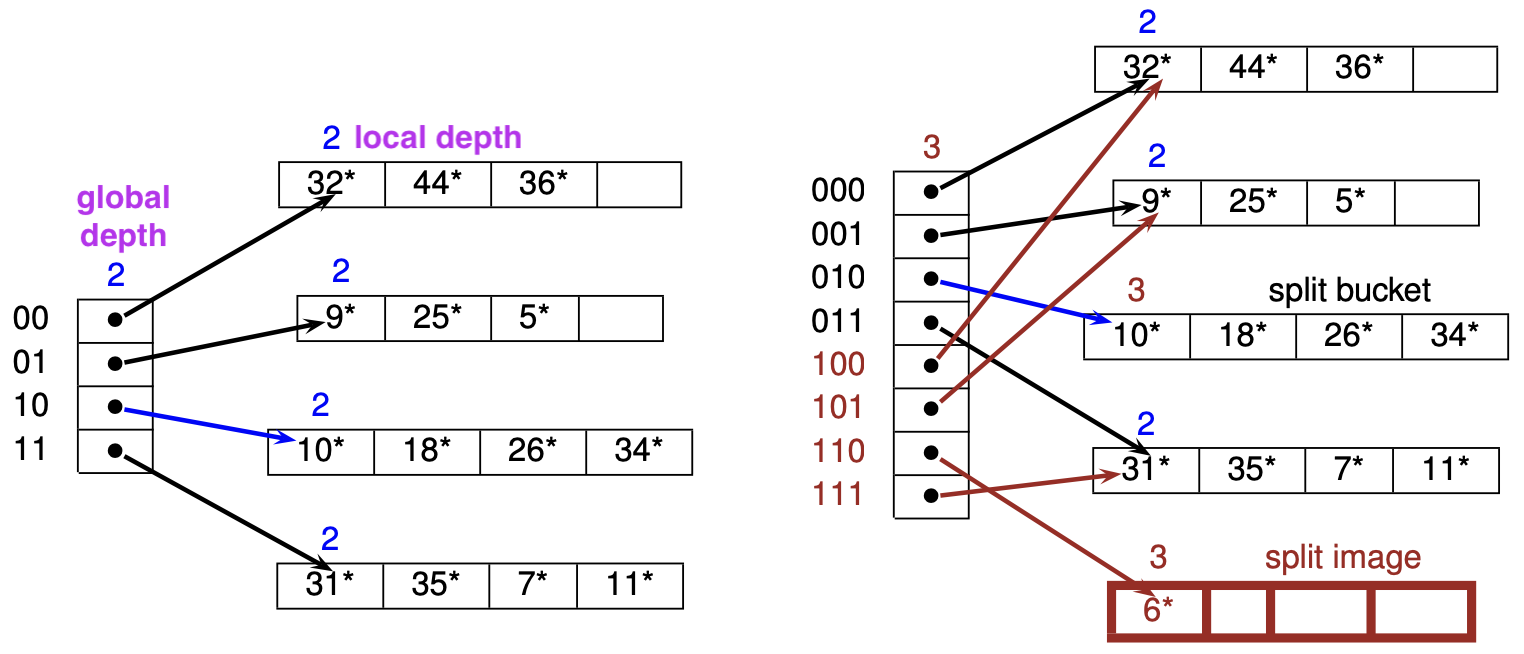
\includegraphics[width=0.95\linewidth]{cs3223-extendible-hashing.png} 
    \item splitting bucket: $\ell$\texttt{++} (repeat until no more overflow)
      \begin{itemize}
        \item if $\ell = d$: directory doubles; $\quad d$\texttt{++}
        \item else $\ell < d$: redistribute and increment $\ell$
      \end{itemize}
    \item deletion: if bucket $B_i$ becomes empty or $B_i$ and $B_j$ can merge,
      \begin{itemize}
        \item deallocate $B_i$ and decrement $\ell$\texttt{-{}-} for split image $B_j$
        \item if each pair of corresponding entries point to the same bucket, the directory can be halved
      \end{itemize}
    \item \textbf{performance}: at most 2 disk I/Os (for equality query)
    \item collisions: when 2 data entries have the same hashed value
      \begin{itemize}
        \item use \textbf{overflow pages} if \# collisions exceeds page capacity
      \end{itemize}
  \end{itemize}

  \section{04.1 SORTING}

  \subsection{External Merge Sort}

  \begin{itemize}
    \item \definition{sorted run} sorted data records written to a file on disk
    \item $N_0 = \left\lceil N/B \right\rceil $
    \item $\text{Num of passes} = \left\lceil \log_{B-1}N_0 \right\rceil + 1$
    \item divide and conquer
      \begin{enumerate}
        \item create temporary file $R_i$ for each $B$ pages of $R$ sorted
        \item merge: use $B-1$ pages for input, 1 page for output
      \end{enumerate}
    \item total I/O = $2N(\lceil \log_{B-1}(N_0) \rceil +1)$
      \begin{itemize}
        \item $2N$ to create $\lceil N/B \rceil $ sorted runs of $B$ pages each
        \item merging sorted runs: $2N \times \lceil \log_{B-1}N_0 \rceil $
      \end{itemize}
  \end{itemize}

  \subsubsection{optimisation with blocked I/O}

  \begin{itemize}
    \item sequential I/O - read/write in \textit{buffer blocks} of $b$ pages
    \item one block ($b$ pages) for output, remaining blocks for input
  \end{itemize}
  \begin{minipage}[c]{0.6\linewidth}{\textcolor{black}{
        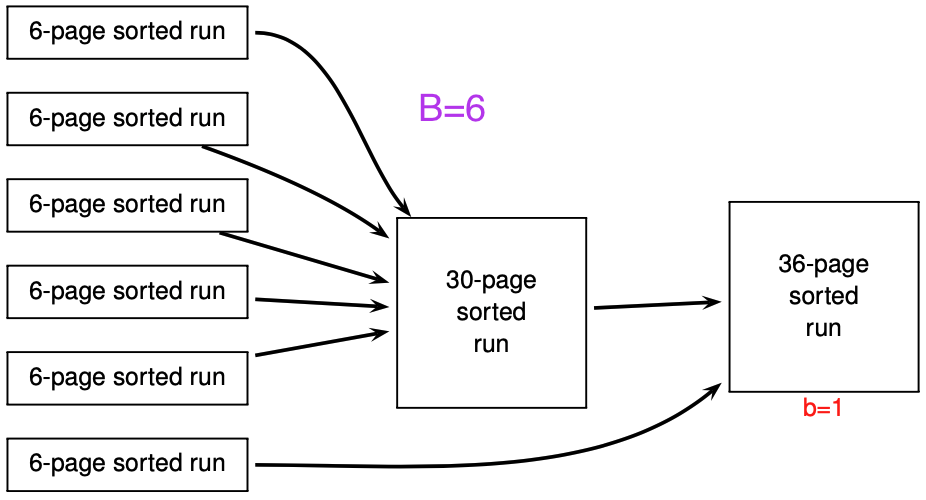
\includegraphics[width=0.97\linewidth]{cs3223-blocked-io-mergesort.png} 
    }}
  \end{minipage}
  \begin{minipage}[c]{0.35\linewidth}
    \begin{itemize}
      \item number of runs merged per pass, \\* $F = \lfloor \frac{B}{b} \rfloor -1$ 
      \item number of passes = $\lceil \log_F(N_0) \rceil +1$
    \end{itemize}
  \end{minipage}

  \subsubsection{Sorting with B$^+$-trees}

  \begin{itemize}
    \item when \textit{sort key is a prefix of the index key} of the B$^+$-tree
    \item sequentially scan leaf pages of B$^+$-tree
      \begin{itemize}
        \item for Format-2/3, use RID to retrieve data records
      \end{itemize}
  \end{itemize}

  \section{04.2 SELECTION: $\sigma_p(R)$}

  \begin{itemize}
    \item $\sigma_p(R)$: selects rows from relation $R$ satisfying predicate $p$
    \item \textbf{access path}: a way of accessing data records/entries 
      \begin{itemize}
        \item \definition{table scan} scan all data pages
        \item \definition{index scan} scan index pages
        \item \definition{index intersection} combine results from index scans 
      \end{itemize}
    \item \definition[of an access path]{selectivity} number of index \& data pages retrieved to access data records/entries
      \begin{itemize}
        \item more selective = fewer pages retrieved
      \end{itemize}
    \item index $I$ is a \definition[for query $Q$]{covering index} if all attributes referenced in $Q$ are part of the key or include cols of $I$ 
      \begin{itemize}
        \item $Q$ can be evaluated using $I$ without any RID lookup (\ildefinition{index-only} plan)
      \end{itemize}
  \end{itemize}

  \subsection{Matching Predicates}

  \begin{itemize}
    \item \definition{term} of form $R.A \;\mathrm{op}\; c$ or $R.A_i \;\mathrm{op}\; R.A_j$
    \item \definition{conjunct} one or more terms connected by $\lor$
      \begin{itemize}
        \item \definition[conjunct]{disjunctive} contains $\lor$
      \end{itemize}
    \item conjunctive normal form, \definition{CNF predicate} comprises one or more conjuncts connected by $\land$
      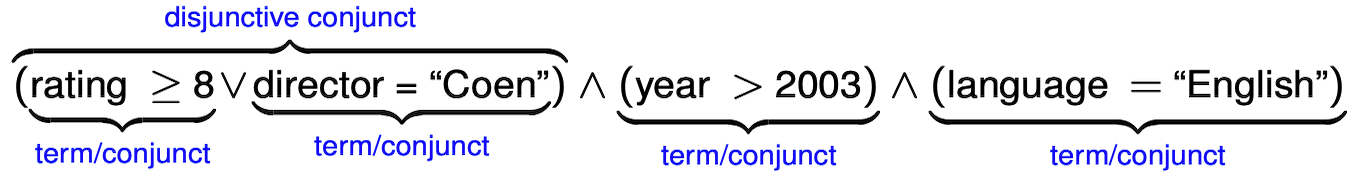
\includegraphics[width=0.95\linewidth]{cs3223-cnf-predicate.png} 
  \end{itemize}

  \subsubsection{B$^+$-tree matching predicates}

  \begin{itemize}
    \item for index $I=(K_1, K_2, \dots, K_n)$ and non-disjunctive CNF predicate $p$, $I$ matches $p$ if $p$ is of the form 
      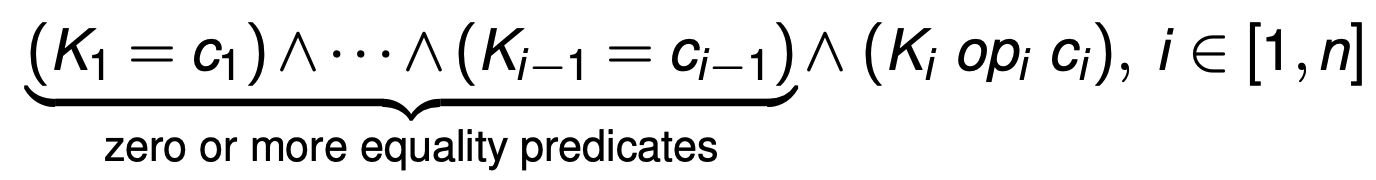
\includegraphics[width=0.9\linewidth]{cs3223-btree-matching-predicate.png} 
      \begin{itemize}
        \item \textit{at most one} non-equality comparison operator which must be on the last attribute of the prefix ($K_i$)
      \end{itemize}
    \item matching index: matching records are in contiguous pages
      \begin{itemize}
        \item non-matching index: not contiguous $\Rightarrow$ less efficient
      \end{itemize}
  \end{itemize}

  \subsubsection{Hash index matching predicates}

  \begin{itemize}
    \item for hash index $I = (K_1, K_2, \dots, K_n)$ and non-disjunctive CNF predicate $p$, $I$ matches $p$ if $p$ is of form 
  \end{itemize}
  \begin{tightcenter}
    \( {\displaystyle{ \quad (K_1=c_1) \land (K_2=c_2) \land \dots \land (K_n=C_n) }} \) 
  \end{tightcenter}

  \subsection{Primary/Covered Conjuncts}

  \begin{itemize}
    \item \definition{primary conjuncts} subset of conjuncts that $I$ matches
      \begin{itemize}
        \item e.g. $p$ = \textcolor{blue}{(age $\geq$ 18) $\land$ (age $\leq$ 20)} $\land$ (weight=65) 
          \\* for $I=$ (age, weight, height)
      \end{itemize}
    \item \definition{covered conjuncts} subset of conjuncts covered by $I$
      \begin{itemize}
        \item each attribute in covered conjuncts appears in key or include cols of $I$
      \end{itemize}
    \item primary conjuncts $\subseteq$ covered conjuncts
  \end{itemize}

  \subsection{Cost of Evaluation}

  let $p'$ = primary conjuncts of $p$, $\quad p_c$ = covered conjuncts of $p$

  \subsubsection{B$^+$-tree index evaluation of p}

  \begin{enumerate}
    \item navigate internal nodes to find first leaf page
      \( {\displaystyle{ 
          \text{cost}_{\text{internal}}=
          \begin{cases}
            \lceil \log_F ( \lceil \frac{||R||}{b_d} \rceil )\rceil &\text{if $$I$$ is a format-1 index}\\
            \lceil \log_F ( \lceil 
            \frac{||R||}{b_i} \rceil )\rceil  &\text{otherwise}
          \end{cases}
      }} \) 
    \item scan leaf pages to access all qualifying data entries
      \( {\displaystyle{ 
          \text{cost}_{\text{leaf}}=
          \begin{cases}
            \lceil \frac{||\sigma_{p'}(R)||}{b_d} \rceil &\text{if $$I$$ is a format-1 index}\\
            \lceil \frac{||\sigma_{p'}(R)||}{b_i} \rceil &\text{otherwise}
          \end{cases}
      }} \) 
    \item retrieve qualified data records via RID lookups
      \( {\displaystyle{ 
          \text{cost}_{\text{RID}}=
          \begin{cases}
            0 &\text{if $$I$$ is a covering format-1 index,}\\
            ||\sigma_{p_c}(R)||  &\text{otherwise}
          \end{cases}
      }} \) 
      \begin{itemize}
        \item reduce cost with \textbf{clustered} data records (sort RIDs): 
          $\lceil\frac{||\sigma_{p_c}(R)||}{b_d}\rceil \leq \text{cost}_{RID} \leq \min\{||\sigma_{p_c}(R)||, |R|\}$
      \end{itemize}
  \end{enumerate}

  \subsubsection{hash index evaluation of p}

  \begin{itemize}
    \item \textbf{format-1}: $\quad$ cost to retrieve data records $ \geq \lceil\frac{||\sigma_{p'}(R)||}{b_d}\rceil $
    \item \textbf{format-2}: $\quad$ cost to retrieve data entries $ \geq \lceil\frac{||\sigma_{p'}(R)||}{b_i}\rceil $ 
      \\* cost to retrieve data records = $ \begin{cases} 0 \quad \text{if $$I$$ is a covering index,}\\
        ||\sigma_{p_c}(R)||  \quad \text{otherwise}
      \end{cases} $
  \end{itemize}


  \section{05.1 PROJECTION $\pi_{A_1, \dots, A_m}(R)$}

  \begin{itemize}
    \item $\pi_L(R)$ eliminates duplicates, $\pi^*_L(R)$ preserves duplicates
  \end{itemize}

  \subsection{Sort-based approach}

  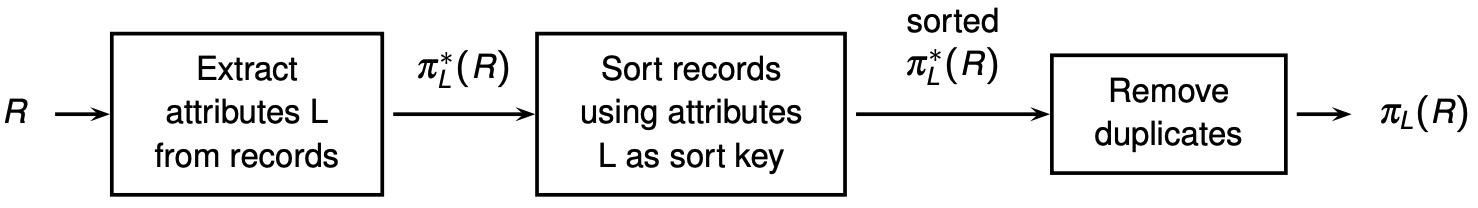
\includegraphics[width=0.95\linewidth]{cs3223-projection-sort-approach.png} 

  \textbf{cost analysis}

  \begin{enumerate}
    \item extract attributes: $|R|$ scan + $\vert \pi^*_L(R)\vert$ output temp result
    \item sort records: $2\vert \pi^*_L(R) \vert (\log_m(N_0) +1)$
    \item remove duplicates: $\vert \pi^*_L(R)\vert$ to scan records
  \end{enumerate}

  \textbf{optimised sort-based approach}

  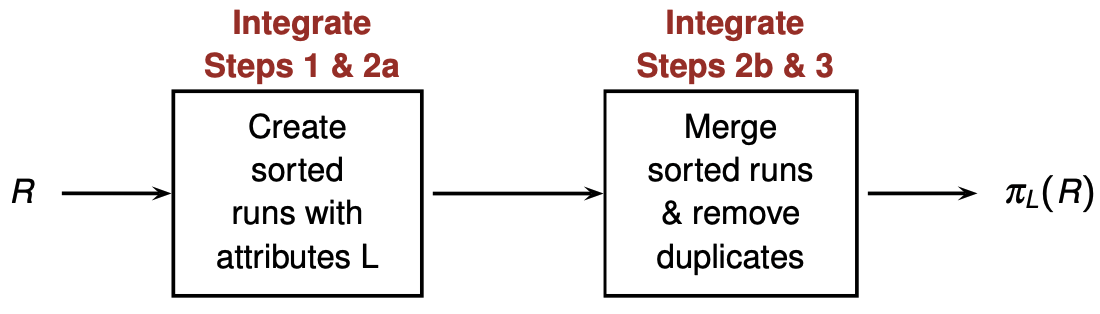
\includegraphics[width=0.8\linewidth]{cs3223-projection-sort-approach-optimised.png} 

  \begin{itemize}
    \item if $B>\sqrt{|\pi^*_L(R)|}$, same I/O cost as hash-based approach
      \begin{itemize}
        \item $N_0 = \lceil \frac{|R|}{B} \rceil \approx \sqrt{|\pi^*_L(R)|}$ initial sorted runs 
        \item $\log_{B-1}(N_0) \approx 1$ merge passes
      \end{itemize}
  \end{itemize}

  \subsection{Hash-based approach}

  \begin{enumerate}
    \item \textbf{partitioning phase}: hash each tuple $t \in R$ 
      \begin{itemize}
        \item $R = R_1 \cup R_2 \cup \dots \cup R_{B-1}$
          \begin{itemize}
            \item for each $R_i$ \& $R_j$, $i \neq j$, $\pi_L^*(R_i) \cap \pi_L^*(R_j) = \emptyset$
          \end{itemize}
        \item for each $t$: project attributes to form $t'$, hash $h(t')$ to one output buffer, flush output buffer to disk when full
        \item one buffer for input, $(B-1)$ buffers for output
      \end{itemize}
    \item \textbf{duplicate elimination} from each partition $\pi^*_L(R_i)$
      \begin{itemize}
        \item for each $R_i$: initialise in-mem hash table, hash each $t \in R_i$ to bucket $B_j$ with $h' \neq h$, insert if $t \not\in B_j$
        \item write tuples in hash table to results
      \end{itemize}
  \end{enumerate}
  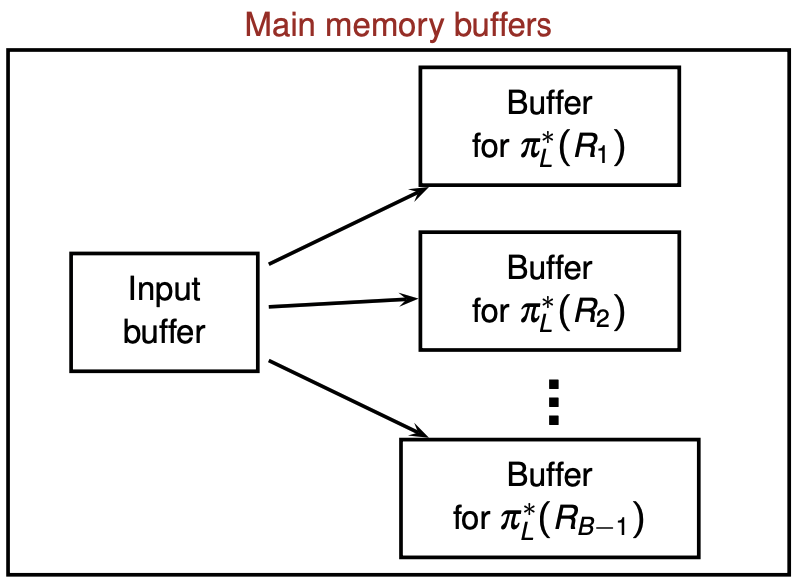
\includegraphics[width=0.4\linewidth]{cs3223-projection-hash-1.png} 
  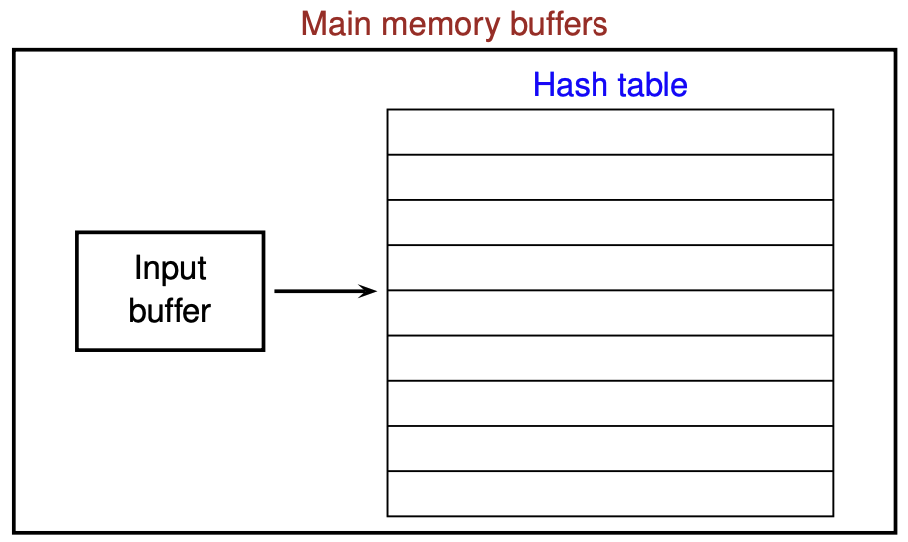
\includegraphics[width=0.5\linewidth]{cs3223-projection-hash-2.png} 

  \begin{itemize}
    \item \textbf{I/O cost} (no partition overflow): $|R| + 2|\pi^*_L(R)|$
      \begin{itemize}
        \item partitioning cost: $|R| + |\pi^*_L(R)|$
        \item duplicate elimination cost: $|\pi^*_L(R)|$
      \end{itemize}
    \item partition overflow: recursively apply partitioning
      \begin{itemize}
        \item to avoid, $B>$ size of hash table for $R_i$ = $\frac{|\pi^*_L(R)|}{B - 1} \times f$
          \begin{itemize}
            \item  approximately $B> \sqrt{f\times |\pi^*_L(R)|}$
          \end{itemize}
          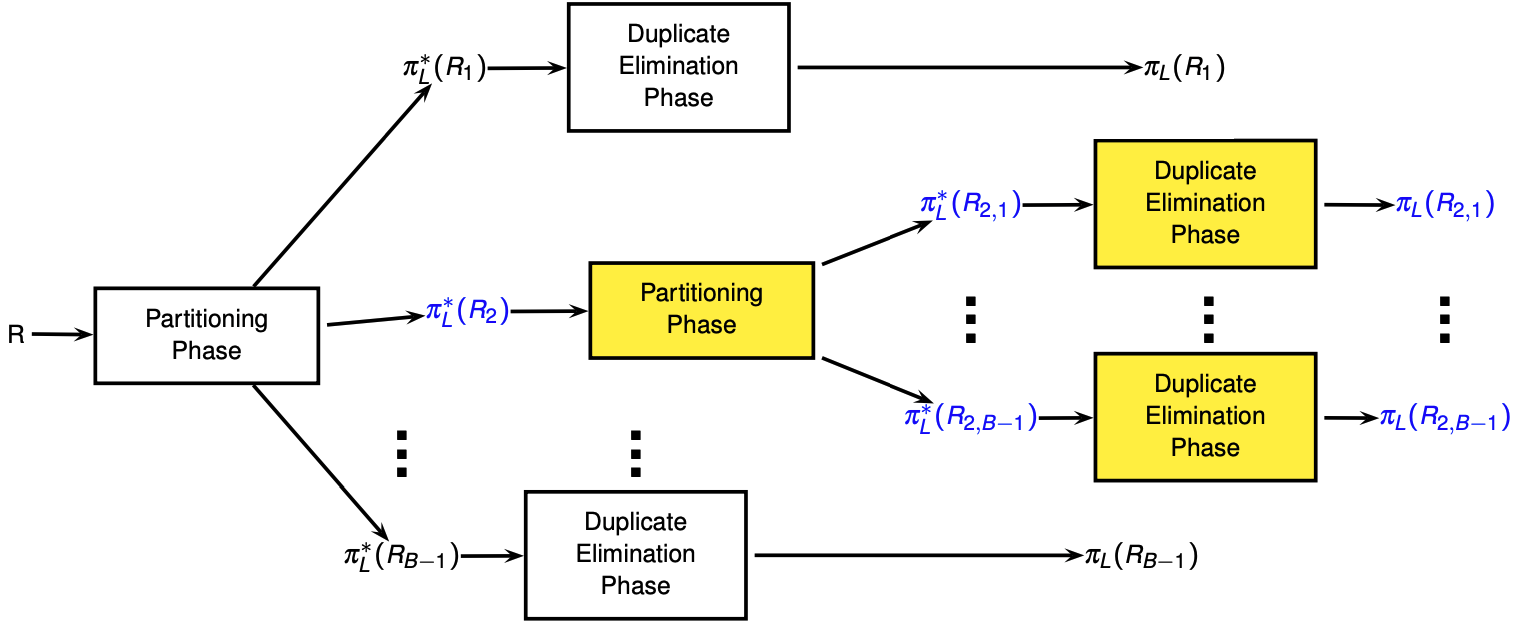
\includegraphics[width=0.9\linewidth]{cs3223-projection-hash-partition-overflow.png} 
      \end{itemize}
  \end{itemize}

  \subsection{Projection using Indexes}

  \begin{itemize}
    \item if index search key contains all wanted attributes \textit{as a prefix}
      \begin{itemize}
        \item \textbf{index scan} data entries in order \& eliminate duplicates
      \end{itemize}
  \end{itemize}

  \section{05.2 JOIN $R \bowtie_\theta S$}

  $R$ = outer relation (smaller relation); $\quad S$ = inner relation

  \attention for \textbf{format-2} index, add cost of retrieving record

  \subsection{nested loop joins and UDA}

  \begin{itemize}
    \item \textbf{tuple-based} nested loop join: $|R| + ||R|| \times |S|$
    \item \textbf{page-based} nested loop join: $|R| + |R| \times |S|$
    \item \textbf{block nested loop join}: $|R| + ( \lceil \frac{|R|}{B-2} \rceil \times |S| )$, $\;\; |R|\leq|S|$
      \begin{itemize}
        \item 1 page output, 1 page input, $(B-2)$ pages to read $R$
        \item for each $(B-2)$ pages of $R$: for each $P_S$ of $S$: check r,s
      \end{itemize}
    \item \textbf{index nested loop join}: \\$|R| + ||R|| \times \left( \underbrace{\log_F(\lceil \frac{||S||}{b_d} \rceil )}_{\text{internal nodes}} + \underbrace{\lceil \frac{||S||}{b_d ||\pi_{B_j}(S)||} \rceil}_{\text{leaf nodes}} + \underbrace{c}_{\text{lookup}}  \right)$
      \begin{itemize}
        \item joining $R(A, B) \bowtie_A S(A,C)$ with B+tree index on $S.A$
        \item for each tuple $r \in R$, use $r$ to probe $S$'s index for match
      \end{itemize}
  \end{itemize}

  \begin{itemize}
    \item In a $B^+$ tree or Hash Index, assume each leaf/bucket has same amount of entries
    \item If $R \Join_{R.a = S.b} S$ and $S.b$ is the primary key. Assume each $S$ tuple joins with $||R||/||S||$ tuples
  \end{itemize}

  \section{NOTATION}

  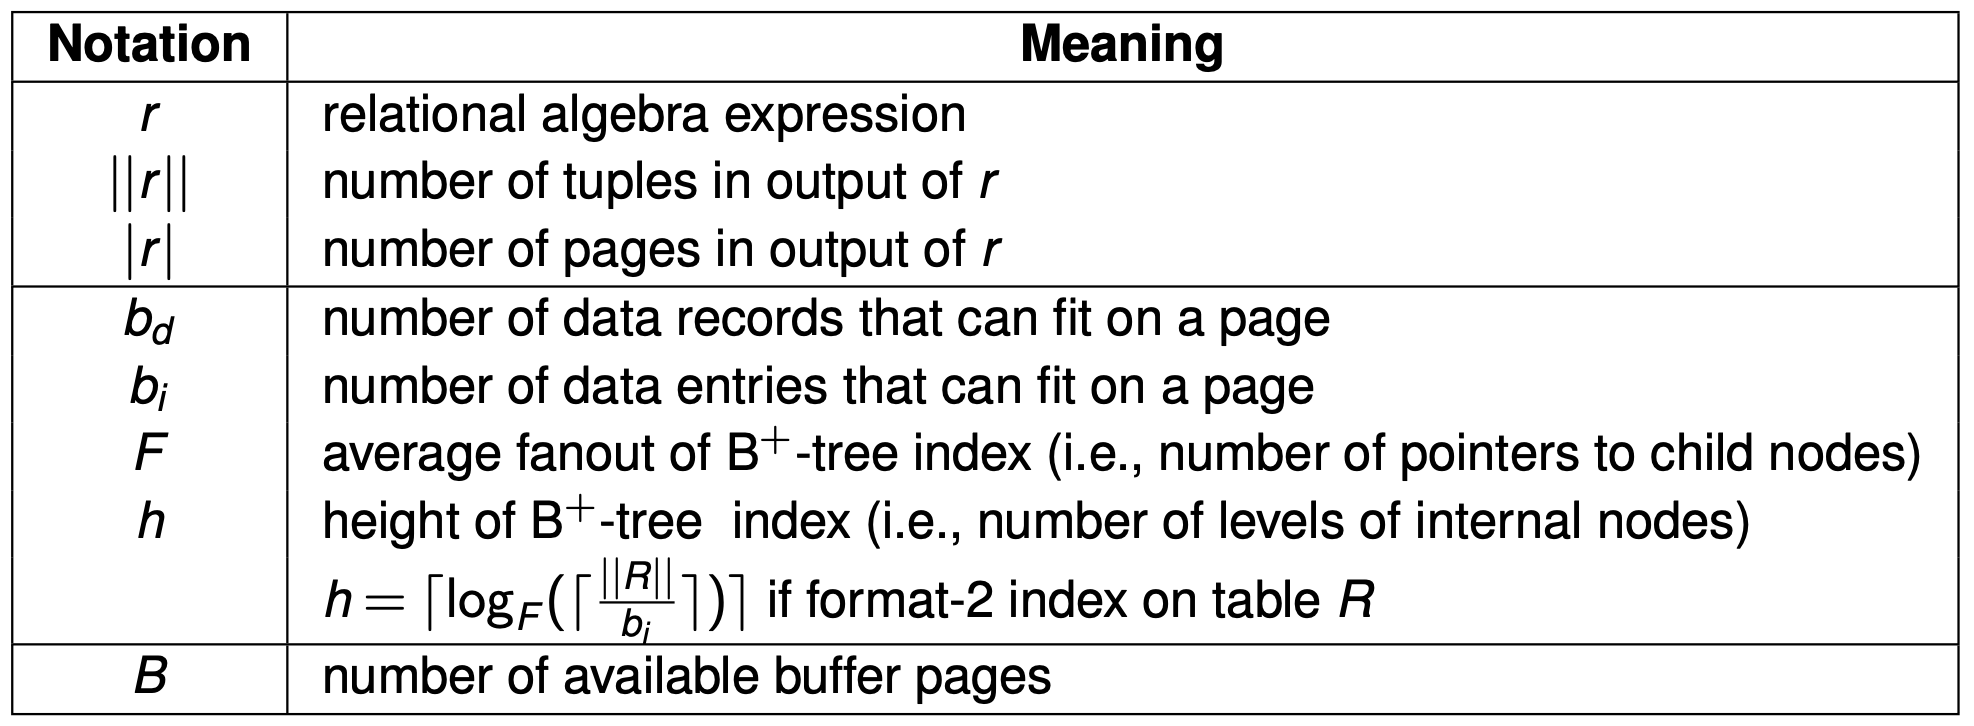
\includegraphics[width=0.97\linewidth]{cs3223-notation.png} 






\end{multicols*}

\end{document}
